\chapter{Modelo Espaço-Temporal aplicado ao GeoGuide}
\label{chap:modelo}

\todo{"Você precisa definir primeiramente um polígono através de imagens"}

\todo{"Através de uma sequência de imagens, mostre como você usa o conceito de polígonos para crir as IDRs e depois sobrepor durante o tempo para identificar as diferências"}

Neste capítulo, explica-se o que são as chamadas Regiões Densas Interessantes e define-se o modelo espaço-temporal e sua aplicabilidade.

\section{Regiões Densas Interessantes}

\abrv[IDR -- Interesting Dense Region]{}

Uma Região Densa Interessante (do inglês {\em Interesting Dense Region}, IDR) é uma região espacial com uma alta probabilidade de conter pontos de interesse do analista. IDRs são coletadas e definidas durante o processamento do feedback do usuário. Diferentemente da literatura que predominantemente foca em interações explícitas, como clicar no botão, esta proposta investiga o feedback implícito.

Durante a exploração iterativa de dados espaciais, é comum o caso que o analista avalia algumas regiões de interesse, mas esquece de dar um feedback explícito sobre aquela região. O ato do usuário olhar para essa região pode ser capturado através do rastreio drastreio dos movimentos oculares e, como \citeonline{arapakis2014user} comprova, esse método possui uma forte relação com a atenção do usuário.

Entretanto, o rastreamento dos movimentos oculares fere várias questões de privacidade. Assim sendo, foi adotado a alternativa de rastrear os deslocamentos do cursor do mouse. \citeonline{arapakis2014understanding} argumenta que esse método possui uma forte relação com o engajamento do usuário. Intuitivamente, um ponto espacial recebe um feedback positivo se o cursor do mouse se desloca próximo a ele frequentemente.

O objetivo de descobrir IDRs é para obter as preferências do analista que nunca foram expressadas explicitamente. Para tal, leva-se em consideração dois conceitos:

\begin{itemize}
	\item \textbf{Conceito 1}: uma região é mais intferessante ao analista, se for densa, ou seja, o analista movimenta seu mouse naquela região várias vezes.
	\item \textbf{Conceito 2}: é possível que o analista movimente seu mouse em qualquer lugar do mapa. Isso não deve significar que todo lugar no mapa tem a mesma relevância.
\end{itemize}

Com base nesses conceitos, o processo de descobrimento das IDRs pode ser descrito pelo Algoritmo \ref{algo:idr}. Pontos são adicionados em $\mathcal{M}$ a cada $200ms$ para evitar pontos redundantes. De acordo com Conceito 1 e com o propósito de identificar comportamentos recorrentes, o algoritmo começa particionando $\mathcal{M}$ em $g$ segmentos consecutivos $\mathcal{M_0}$ até $\mathcal{M_g}$. O primeiro segmento começa no momento zero (quando a iteração iniciou) e o último termina em $t_c$, ou seja, no tempo atual que o algoritmo é executado. De acordo com o Conceito 2, formam-se os clusters em cada segmento de $\mathcal{M}$ usando uma variação da abordagem DB-SCAN \cite{Ester:1996}. Por fim, as interseções desses clusters são encontradas e retornadas como IDRs.

\begin{algorithm}[t]
	\DontPrintSemicolon
	\KwIn{Tempo atual $t_c$, pontos dos movimentos do mouse $\mathcal{M}$}
	\KwOut{IDRs encontradas $\mathcal{S}$}
	$\mathcal{S} \gets \emptyset$\;
	$g \gets ${\em número de segmentos}\;
	\For{$i \in [0,g]$}
	{
		   $\mathcal{M}_i \gets \{m = \langle x,y,t \rangle | (\frac{t_c}{g} \times i) \leq t \leq (\frac{t_c}{g} \times (i+1))\}$\;
		   $\mathcal{C}_i \gets \mathit{mine\_clusters}(\mathcal{M}_i)$\label{ln:mine}\;
		   $\mathcal{O}_i \gets \mathit{find\_polygons}(\mathcal{C}_i)$\label{ln:poly}\;
	}
	\lFor{$\mathcal{O}_i, \mathcal{O}_j$ onde $i,j \in [0,g]$ e $i \neq j$}
	{
		   $\mathcal{S}.\mathit{append}(\mathit{intersect}(\mathcal{O}_i, \mathcal{O}_j))$
	}
	% $\mathcal{H} \gets \mathit{discover\_highlights}(\mathcal{S},k)$\label{ln:geoguide}\;
	\Return{$\mathcal{S}$}\; 
	\caption{Descobrimento de IDRs}
	\label{algo:idr}
\end{algorithm}

Para clusterizar os pontos em cada segmento de tempo (linha \ref{ln:mine} do Algoritmo \ref{algo:idr}), é utilizado o ST-DBSCAN, uma variação do DB-SCAN que leva em consideração atributos espaciais e temporais para clusterizar pontos com base na densidade \cite{Birant:2007}. Para cada subconjunto de pontos dos movimentos do mouse $\mathcal{M}_i$, $i \in [0,g]$, ST-DBSCAN começa com um ponto aleatório $m_0 \in \mathcal{M}_i$ e coleta todos os pontos alcançaveis (de acordo com a densidade) de $m_0$ usando uma métrica de distância. Como os pontos dos movimentos do mouse ocorrem em um espaço bidimensional (monitor do computador), a distância euclidiana foi selecionada como métrica. Se $m_0$ for identificado como objeto {\em core}, uma cluster será gerado. Caso contrário, se $m_0$ é uma objeto de borda, nenhum ponto é alcançável de $m_0$ e o algoritmo buscará outro ponto aleatório em $\mathcal{M}_i$. Esse processo é repetido até que todos os pontos sejam processados.

Uma vez que os clusters são formados para cada subconjunto de $\mathcal{M}$, encontra-se suas interseções para determinar as regiões recorrentes. Para obter as interseções é preciso definir nitidamente as fronteiras dos clusters (linha \ref{ln:poly}). Portanto para cada cluster, é construído seu respectivo polígono que engloba todos os pontos. Para isso, é utilizado o algoritmo Quickhull, um método com abordagem similar ao Quicksort, que calcula o invólucro convexo para um determinado conjunto de pontos num plano bidimensional \cite{Barber:1996}.

Esse algoritmo de descoberta de IDR é executado a cada $t$ intervalo de tempo durante uma análise exploratória. Dessa forma, enquanto o analista está explorando o conjunto de dados, suas preferências estão sendo coletadas continuamente. Na Figura \ref{fig:descoberta-idr}, observa-se uma iteração de coleta e execução desse algoritmo onde $g = 3$, ou seja, o feedback é coletado em 3 segmentos diferentes de tempo. Os movimentos do mouse realizados pelo analista nesses 3 segmentos são demonstrados na Figura \ref{fig:descoberta-idr}.A. Para cada segmento, os pontos coletados dos movimentos do mouse são clusterizados e convertidos em polígonos convexos (Figura \ref{fig:descoberta-idr}.B-D, respectivamente). Por fim, os polígonos são sobrepostos (Figura \ref{fig:descoberta-idr}.E) e as interseções encontradas são definidas como IDRs (IDR1-4 na Figura \ref{fig:descoberta-idr}.F).

\begin{figure}[t]
	\centering
	\includegraphics[width=\textwidth]{imagens/regions}
	\caption{Processo de descoberta de IDRs}
	\label{fig:descoberta-idr}
\end{figure}

% Há diversas abordagem para inferir uma região espacial para um determinado conjunto de pontos \cite{Bevis1989,DUCKHAM2008,FADILI2004,ARAMPATZIS2006,Galton2006}. A abordagem comum é agregar os pontos na forma de polígonos côncavos e convexos. Na construção de um polígono côncavo, as concavidades de um polígono pode conter pontos que não estão necessariamente presentes em $\mathcal{M}$. No algoritmo de descoberta de IDR, adaptamos o uso do Quickhull \cite{Barber:1996}, por causa da sua simplicidade, eficiência e sua implementação natural de polígonos convexos.

\subsection{Perfil}

Uma IDR descreve uma região espacial no conjunto de dados do analista coletada num determinado tempo $t$. Cada região representa as preferências do analista no momento $t$ no contexto espacial, ou seja, {\em onde} o analista está interessado. Para entender, {\em em que} o analista está interessado, em outras palavras, as preferências sobre o contexto de domínio, é definido o perfil de cada região.

\begin{table}[]
	\centering
	\begin{tabular}{|l|l|}
		\hline
		\textbf{id}                  & 15                             \\ \hline
		\textbf{latitude}            & 48.88880                       \\ \hline
		\textbf{longitude}           & 2.320465                       \\ \hline
		\textbf{name}                & Nice appartment in Batignolles \\ \hline
		\textbf{host\_name}          & Daniele                        \\ \hline
		\textbf{neighbourhood}       & Batignolles-Monceau            \\ \hline
		\textbf{room\_type}          & Entire home/apt                \\ \hline
		\textbf{price}               & 65                             \\ \hline
		\textbf{minimun\_nights}     & 1                              \\ \hline
		\textbf{stars}               & 4                              \\ \hline
		\textbf{number\_of\_reviews} & 25                             \\ \hline
		\textbf{reviews\_per\_month} & 1.74                           \\ \hline
		\textbf{availability\_365}   & 35                             \\ \hline
		\textbf{last\_review}        & 2015-11-14T09:07:02+00:00      \\ \hline
	\end{tabular}
	\caption{Exemplo de atributos de um ponto que representa uma estadia}
	\label{table:atributos}
\end{table}

O perfil é a sumarização dos atributos dos pontos contidos numa IDR. Cada ponto em um conjunto de dados ($p \in \mathcal{P}$) é descrito por suas coordenadas espaciais e uma série de atributos de domínio $dom(p)$. A Tabela \ref{table:atributos} apresenta um exemplo dos atributos de um ponto no conjunto de dados do Airbnb.

Na Tabela \ref{table:atributos}, os atributos {\em latitude} e {\em longitude} são as coordenadas espaciais, enquanto que todos os outros atributos caracterizam os atributos de domínio. Dentre os atributos de domínio pode-se encontrar 4 tipos de dados:

\begin{enumerate}
	\item Numéricos: são atributos que representam valores numéricos, como, por exemplo, os atributos {\em price}, {\em minimun\_nights}, {\em number\_of\_reviews}, {\em reviews\_per\_month} e {\em availability\_365}.
	\item Textuais: são atributos que representam valores textuais, como, por exemplo, os atributos {\em name} e {\em host\_name}.
	\item Categóricos: são atributos que representam valores tanto numéricos quanto textuais, mas que se repetem pouco em todo o conjunto. Por exemplo, o atributo {\em stars} possui apenas cinco valores em todo o conjunto. Os atributos {\em room\_type} e {\em neighbourhood} também possuem um número finito de opções, por isso são classificados como categóricos.
	\item Temporais: são atributos que representam data e/ou hora de um determinado evento, como, por exemplo, o atributo {\em last\_review} que representa quando foi publicado a última avaliação.
\end{enumerate}

Esses 4 tipos de dados são comumente encontrados em conjuntos de dados espaciais, portanto o perfil da IDR precisa representar de maneira resumida esses atributos em relação aos pontos nela contidos. Assim sendo, cada tipo é tradado de acordo com sua especificidade.

O atributos classificados como numéricos encontrados em uma IDR são sumarizados usando funções estatísticas como média, desvio padrão, mínimo e máximo. Observa-se um exemplo do resultado dessa sumarização na Tabela \ref{table:perfil-numericos}.

\begin{table}[!h]
	\centering
	\begin{tabular}{|l|r|r|r|r|r|}
	\hline
	\multicolumn{1}{|c|}{\textbf{Atributo}} & \multicolumn{1}{c|}{\textbf{Total}} & \multicolumn{1}{c|}{\textbf{Média}} & \multicolumn{1}{c|}{\textbf{$\sigma$}} & \multicolumn{1}{c|}{\textbf{Mínimo}} & \multicolumn{1}{c|}{\textbf{Máximo}} \\ \hline
	price                                   & 73                                       & 106,68                              & 62,62                                       & 40                                   & 401                                  \\ \hline
	minimun\_nights                         & 73                                       & 2,36                                & 1,60                                        & 1                                    & 7                                    \\ \hline
	number\_of\_reviews                     & 73                                       & 17,86                               & 27,85                                       & 0                                    & 120                                  \\ \hline
	reviews\_per\_month                     & 55                                       & 1,64                                & 1,53                                        & 0,08                                 & 7,27                                 \\ \hline
	calculated\_host\_listings\_count       & 73                                       & 4,05                                & 10,83                                       & 1                                    & 56                                   \\ \hline
	availability\_365                       & 73                                       & 179,64                              & 154,48                                      & 0                                    & 365                                  \\ \hline
	\end{tabular}
	\caption{Exemplo de perfil dos atributos numéricos de uma IDR}
	\label{table:perfil-numericos}
\end{table}

Os atributos textuais são tratados individualmente. Para cada atributo é feito o levantamento dos termos mais usados. Essa abordagem é utilizada por \citeonline{kumar2017} para encontrar os termos mais frequentes no contexto temporal. A Tabela \ref{table:perfil-textual} apresenta os 5 primeiros resultados para o atributo {\em name} em uma IDR.

\begin{table}[!h]
	\centering
	\begin{tabular}{|l|r|}
	\hline
	\multicolumn{2}{|c|}{\textbf{Atributo: name}} \\ \hline
	\textbf{Termo}     & \textbf{Ocorrências}     \\ \hline
	champs             & 29                       \\ \hline
	elysées            & 18                       \\ \hline
	studio             & 14                       \\ \hline
	near               & 13                       \\ \hline
	flat               & 11                       \\ \hline
	\end{tabular}
	\caption{Exemplo parcial de perfil do atributo textual de uma IDR}
	\label{table:perfil-textual}
\end{table}

Os atributos categóricos são contabilizados num dicionário $C$ onde as chaves são uma tupla com o nome do atributo e o valor da categoria. Quanto maior a quantidade de repetições de uma categoria, mais relevante essa categoria é no contexto de uma IDR. A Tabela \ref{table:perfil-categoricos} mostra o resultado num conjunto de dados para os atributos {\em neighbourhood}, {\em room\_type} e {\em stars}.

\begin{table}[!h]
	\centering
	\begin{tabular}{|l|r|}
	\hline
	\textbf{Categoria}                                            & \textbf{Quantidade} \\ \hline
	\textless{}neighbourhood, "Batignolles-Monceau"\textgreater{} & 73                  \\ \hline
	\textless{}room\_type, "Entire home/apt"\textgreater{}        & 69                  \\ \hline
	\textless{}room\_type, "Private room"\textgreater{}           & 4                   \\ \hline
	\textless{}stars, 1\textgreater{}                             & 6                   \\ \hline
	\textless{}stars, 2\textgreater{}                             & 7                   \\ \hline
	\textless{}stars, 3\textgreater{}                             & 29                  \\ \hline
	\textless{}stars, 4\textgreater{}                             & 20                  \\ \hline
	\textless{}stars, 5\textgreater{}                             & 11                  \\ \hline
	\end{tabular}
	\caption{Exemplo de perfil dos atributos categóricos de uma IDR}
	\label{table:perfil-categoricos}
\end{table}

Os atributos temporais são normalizados para uma escala linear (a partir do ano novo para datas e a partir da meia noite para horas) objetivando contabilizar as ocorrências. Por exemplo, um atributo com a data {\em 2018-12-21} é normalizado para {\em 2018, 12, 355}, isto é, numa linha temporal esse evento ocorreu no ano 2018, no 12º mês e no 355º dia. As horas são normalizadas de maneira similar, a hora {\em 08:33:22} é normalizada para {\em 8, 513, 30802}, isto é, esse evento ocorreu na 8º hora, 513º minuto e 30802º segundo. Com os valores normalizadas, pode-se encontrar os dias e os momentos do dia mais recorrentes para determinado evento em uma IDR.

\todo{adicionar algoritmo(?)}

\section{Análise de Variação Temporal}

Cada IDR é coletada num momento $t$ e seu perfil definido através dos atributos de domínio dos pontos contidos na região delimitada. Apesar do perfil ser definido para cada IDR, pode também ser definido para um conjunto de IDRs, ou seja, se num momento $t$ houver 3 IDRs, é possível combinar os pontos contidos nessas regiões e definir um perfil para esse momento $t$. 

Em outras palavras, é possível realizar a análise das preferências do analista em qualquer espaço de tempo (seja minutos ou dias, semanas ou meses), uma vez que o sistema coleta as preferências do usuário de maneira transparente enquanto o mesmo realiza a análise exploratória do conjunto de dados. Dessa forma, para cada momento $t$ em qualquer espaço de tempo, pode-se detectar as preferências do usuário tanto no contexto espacial, quanto no contexto de domínio.

\subsection{Contexto Espacial}

O contexto espacial se refere aos aspectos geográficos como, por exemplo, em que parte da cidade o analista se interessa. A Figura \ref{fig:analise-contexto-espacial} apresenta as regiões encontradas em 3 momentos sequenciais, sendo \ref{fig:analise-contexto-espacial}.C o mais recente. É possível abordar o contexto espacial em, ao menos, 3 aspectos: deslocamento, distância e área.

\begin{figure}[]
	\centering
	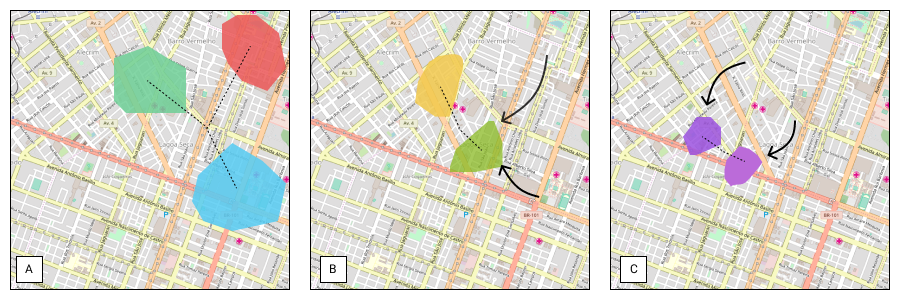
\includegraphics[width=\textwidth]{imagens/analise-contexto-espacial}
	\caption{Evolução no contexto espacial}
	\label{fig:analise-contexto-espacial}
\end{figure}

\subsubsection{Deslocamento de IDR}

Identificar padrões no deslocamento das IDRs pode ser eficiente para entender o processo que o analista realizou para resolver determinada tarefa. Com esse conhecimento, o sistema pode otimizar a análise exploratória para o analista numa tarefa similar ou para outros analistas que estejam realizando a mesma tarefa. Por exemplo, na Figura \ref{fig:analise-contexto-espacial}, os padrões de deslocamento estão indicados pelas setas curvilíneas. No primeiro momento (\ref{fig:analise-contexto-espacial}.A), naturalmente não é possível identificar uma movimentação, mas as regiões encontradas nesse momento servem como ponto de partida da análise. No segundo momento (\ref{fig:analise-contexto-espacial}.B), percebe-se um deslocamento: o analista, que antes explorou regiões ao norte, norteste e oeste, agora tem sua atenção voltada para o norte e centro-oeste. Já no terceiro momento (\ref{fig:analise-contexto-espacial}.B), pode-se identificar um padrão de deslocamento para região central.

\subsubsection{Distância entre IDRs}

A distância entre as IDRs, indicadas na Figura \ref{fig:analise-contexto-espacial} pelas retas tracejadas do centro de cada região até o centro do conjunto, revela o quão distribuido está a análise do usuário. Na Figura \ref{fig:analise-contexto-espacial}.A, ponto de partida da análise, o analista não sabe exatamente onde procurar, então ele avalia várias regiões na cidade, resultando em conjunto de IDRs bem distribuído. Com o passar das iteraçãos, o espaço de procura do analista tende a diminuir, ou seja, as IDRs identificadas tendem a serem mais próximas como pode ser observado na sequência \ref{fig:analise-contexto-espacial}.B-C.

\subsubsection{Área de IDR}

A área de cada IDR, indicadas na Figura \ref{fig:analise-contexto-espacial} pelos polígonos definidos, indica o quão concentrado está a análise do usuário. No primeiro momento (\ref{fig:analise-contexto-espacial}.A), as áreas das IDRs são consideravelmente maiores, o que pode indicar um comportamento de reconhecimento, ou seja, o analista está realizando um processo de reconhecimento do conjunto de dados a fim de se direcionar para próxima iteração. No segundo momento (\ref{fig:analise-contexto-espacial}.B), as áreas das regiões diminuiram, o que pode apontar que a análise está mais precisa e direcionada. No momento seguinte (\ref{fig:analise-contexto-espacial}.C), é notável a evolução do analista direção ao objetivo da sua tarefa, visto que seu interesse, representado pelas IDRs, está mais concentrado indicando que o analista sabe onde e o qué está procurando.

% \closesubsection

\subsection{Contexto de Domínio}

O contexto de domínio se refere aos aspectos de domínio como, por exemplo, se o analista tem mais interesse em casas com varanda ou apartamentos. A análise é feita considerando os perfis das regiões, ou seja, como os atributos, de cada tipo, são relevantes ao analista ao decorrer das iterações.

% \subsection{Numéricos}
\begin{figure}[]
	\centering
	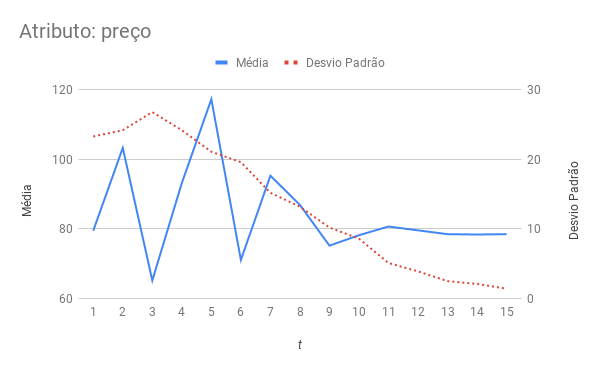
\includegraphics[width=\textwidth]{imagens/analise-atributo-numerico}
	\caption{Evolução de atributo numérico}
	\label{fig:analise-atributo-numerico}
\end{figure}

Os atributos numéricos se apresentam relevantes quando a variação do valor médio tende a zero, assim como seu desvio padrão com o passar das iterações. Por exemplo, na Figura \ref{fig:analise-atributo-numerico}, observa-se que após 11 iterações ($t$), o atributo {\em preço} se mostrou relevante ao analista, uma vez que seu valor médio se tornou linear, em outras palavras, com diferenças mínimas entre as iterações, e seu desvio padrão quase 0.


Diferentemente dos atributos numéricos que podem ser analisados pelas diferenças nas suas estatísticas, os atributos textuais e categóricos precisam ser analisados através de sua evolução no decorrer das iterações. Para tal, contrói-se um vetor de feedback $F$ que é atualizado à cada iteração com base nos perfis das IDRs descobertas.

Considera-se um {\em valor de incremento} $\delta$ para atualizar $F$. Se $v_1$ para atributo $a_1$ é encontrado $x$ vezes na IDR, aumenta-se por $x\delta$ o valor de \textless{}$a_1, v_1$\textgreater{} em $F$. Durante a atualização, os valores em $F$ só podem ser incrementados, ou seja, nunca são diretamente diminuidos.

\begin{table}[!h]
	\centering
	\begin{tabular}{|c|c|}
	\hline
	\textbf{Categoria}                      & \textbf{Quantidade} \\ \hline
	\textless{}Beds, 1\textgreater{}        & 3                   \\ \hline
	\textless{}Beds, 2\textgreater{}        & 1                   \\ \hline
	\textless{}Beds,+2\textgreater{}        & 0                   \\ \hline
	\textless{}Balcony, Yes\textgreater{}   & 4                   \\ \hline
	\textless{}Balcony, No\textgreater{}    & 0                   \\ \hline
	\textless{}Air-cond., Yes\textgreater{} & 1                   \\ \hline
	\textless{}Air-cond., No\textgreater{}  & 3                   \\ \hline
	\textless{}Rating, 1\textgreater{}      & 0                   \\ \hline
	\textless{}Rating, 2\textgreater{}      & 0                   \\ \hline
	\textless{}Rating, 3\textgreater{}      & 0                   \\ \hline
	\textless{}Rating, 4\textgreater{}      & 1                   \\ \hline
	\textless{}Rating, 5\textgreater{}      & 3                   \\ \hline
	\end{tabular}
	\caption{Exemplo de perfil de atributos categóricos}
	\label{table:attribs}
\end{table}

Usando como exemplo o perfil de atributos categóricos apresentado na Tabela \ref{table:attribs} de um conjunto de dados sobre estadias, o vetor de feedback atualizado na primeira iteração pode ser observado na Tabela \ref{table:feedback}. Como o atributo ``Beds'' recebe o valor ``1'' três vezes, o valor da célula \textless{}$Beds, 1$\textgreater{} é incrementado três vezes por $\delta$. O mesmo processo é repetido para todos atributo-valores dos perfis. É importante notar que nem todas as células de $F$ são necessariamente atualizadas durante o processo, como nesse exemplo, 5 células de 12 permaneceram sem atualização.

Por especificar um valor de incremento, é possível atualizar e normalizar o vetor de feedback usando uma função Softmax. $F$ é sempre normalizado de maneira que seus valores somados sejam $1.0$. Sendo $\delta = 1.0$, os valores normalizados do vetor $F$ são ilustrados na terceira coluna da Tabela \ref{table:feedback}. Os maiores valores indicam os atributos mais relevantes.

Os valores normalizados do vetor $F$ representa as preferências do analista. Por exemplo, os valores na Tabela \ref{table:feedback} depois da atualização mostram que o analista tem bastante interesse em ter uma varanda ({\em balcony}) em sua estadia, uma vez que o valor \textless{}$Balcony, Yes$\textgreater{} é 0.25, isto é, o maior. Apesar de apenas considerar diferenças positivas, a função Softmax reduz valores das células que não foram relevantes a cada iteração ao passo que outras células são incrementadas.

É importante frisar que valores ``0'' no vetor $F$ não significa a menor relevância, mas {\em irrelevância}. Por exemplo, considerando a célula \textless{}$Rating, 2$\textgreater{} na Tabela \ref{table:feedback}, o valor ``0'' para essa célula indica que o analista não demostrou interesse nessa característica. É possível que em iterações futuras, o analista demostre interesse em estadias de 2 estrelas (potencialmente por causa do preço), nesse caso o valor dessa célula deixaria de ser 0. Entretanto, células que representam relavâncias menores são identificados com valores que tendem a 0. Por exemplo, o valor 0.06 para célula \textless{}$Rating, 4$\textgreater{} mostra uma preferência por uma estadia de 4 estrelas inferior se comparado com as de 5 estrelas.

\begin{table}[]
	\centering
	\begin{tabular}{|c|c|c|}
	\hline
	\textbf{Atributo-valor}               & \textbf{Atualização} & \textbf{Normalizado} \\ \hline
	\textless{}Beds, 1\textgreater{}                   & $+3\delta$                       & 0.19                 \\ \hline
	\textless{}Beds, 2\textgreater{}                 & $+\delta$                       & 0.06                 \\ \hline
	\textless{}Beds, +2\textgreater{}                  & {\em (sem atualização)}                       & 0.00                    \\ \hline
	\textless{}Balcony, Yes\textgreater{}                   & $+4\delta$                      & {\bf 0.25}                 \\ \hline
	\textless{}Balcony, No\textgreater{}                    & {\em (sem atualização)}                        & 0.00                    \\ \hline
	\textless{}Air-cond., Yes\textgreater{}               & $+\delta$                       & 0.06                 \\ \hline
	\textless{}Air-cond., No\textgreater{}                & $+3\delta$                       & 0.19                 \\ \hline
	\textless{}Rating, 1\textgreater{}                    & {\em (sem atualização)}                       & 0.00                    \\ \hline
	\textless{}Rating, 2\textgreater{}                     & {\em (sem atualização)}                        & 0.00                    \\ \hline
	\textless{}Rating, 3\textgreater{}                    & {\em (sem atualização)}                        & 0.00                   \\ \hline
	\textless{}Rating, 4\textgreater{}                   & $+\delta$                       & {\bf 0.06}                 \\ \hline
	\textless{}Rating, 5\textgreater{}                     & $+3\delta$                      & 0.19                 \\ \hline
	\end{tabular}
	\caption{Atualizando vetor de feedback}
	\label{table:feedback}
\end{table}


O vetor de feedback para atributos textuais difere apenas na sua inicialização. Como os perfis para atributos textuais são construídos separadamente, é preciso combinar os valores de cada atributo no único vetor. Por exemplo, se a frequência das palavras no atributo textual {\em name} é representado na Tabela \ref{table:perfil-textual} e do atributo {\em description} na Tabela \ref{table:perfil-textual-2}, no vetor de feedback haveria células como \textless{}$confort, 33$\textgreater{}, \textless{}$mobilier, 32$\textgreater{} e \textless{}$champs, 29$\textgreater{}, ou seja, as células presentes no vetor contemplam todos os atributos textuais.

\begin{table}[!h]
	\centering
	\begin{tabular}{|l|r|}
	\hline
	\multicolumn{2}{|c|}{\textbf{Atributo: description}} \\ \hline
	\textbf{Termo}     & \textbf{Ocorrências}     \\ \hline
	confort             & 33                       \\ \hline
	mobilier            & 32                       \\ \hline
	appartement             & 22                       \\ \hline
	décoré               & 21                       \\ \hline
	adorable               & 18                       \\ \hline
	\end{tabular}
	\caption{Exemplo parcial de perfil do atributo textual}
	\label{table:perfil-textual-2}
\end{table}

No caso dos atributos temporais, detectar padrões de preferências é mais complicado visto a natureza do dado temporal. A primeira abordagem é intepretar os perfis temporais ao longo das iterações como na Figura \ref{fig:analise-atributo-temporal}, ou seja, como um gráfico de dispersão onde o eixo $x$ são as iterações $t$, o eixo $y$ é a linha temporal dos eventos para determinado atributo e o tamanho do ponto é a frequência do evento. A Figura \ref{fig:analise-atributo-temporal} apresenta os resultados para o atributo {\em last\_review} em um conjunto de dados de estadias após 7 iterações ($t$).

\begin{figure}[!h]
	\centering
	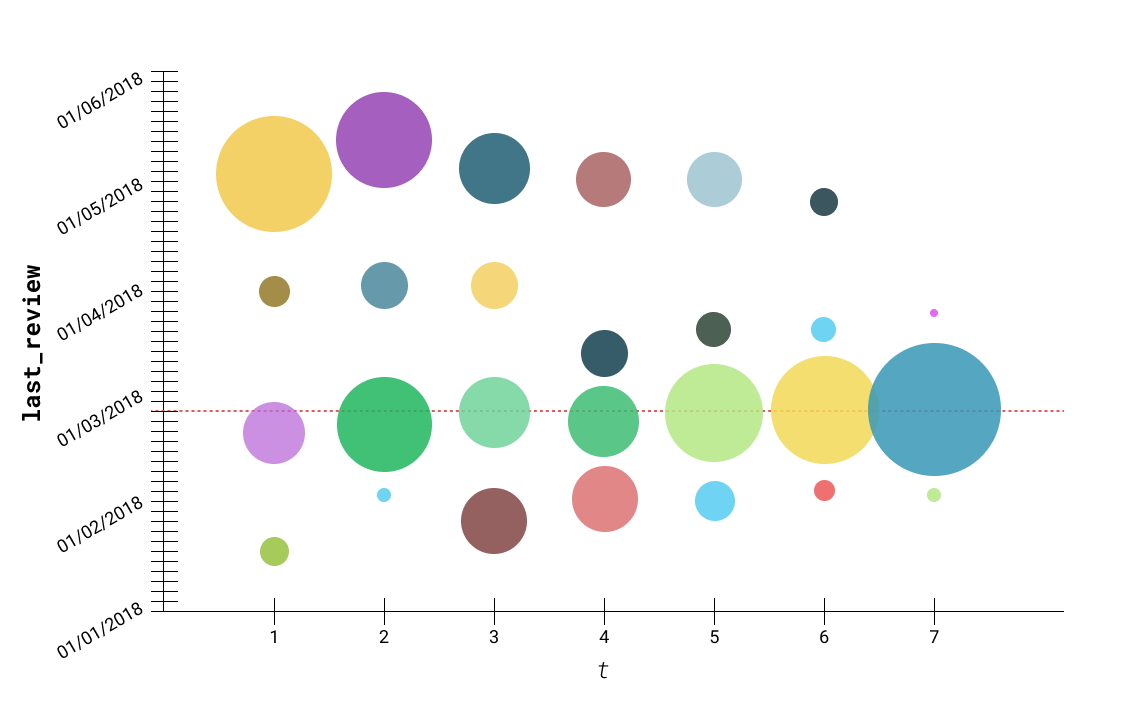
\includegraphics[width=\textwidth]{imagens/analise-atributo-temporal}
	\caption{Evolução de atributo temporal}
	\label{fig:analise-atributo-temporal}
\end{figure}

Nas primeiras iterações ($t <= 4$), pode-se perceber que o analista não demostra nenhum preferência específica para o atributo {\em last\_review}, visto que os dados estão bem destribuídos. A partir da 5º iteração, é notável a concentração do interesse do analista em avaliações ({\em reviews}) enviadas entre final de fevereiro e começo de março.

A segunda abordagem a ser utilizada para identificar padrões de preferências do analista sobre atributos temporais é considerar os valores máximos e mínimos para construir uma janela de interesse. Por exemplo, na Figura \ref{fig:analise-atributo-temporal}, pode-se dizer que a janela de interesse do usuário no evento {\em last\_review} a partir de 7º iteração é 15 de fevereiro de 2018 até 15 de março de 2018, portanto eventos que ocorreram entre essas datas são mais relevantes ao analista.

É importante notar no exemplo da Figura \ref{fig:analise-atributo-temporal} a granularidade da linha temporal do atributo em questão é de dias. A granularidade durante a análise pode ser variável, ou seja, se adequar a janela de interesse do usuário, ou fixa, como nesse exemplo. Isso só é possível de maneira eficiente, pois os atributos temporais são normalizados durante a construção do perfil em 6 granularidade: anos, meses, dias, horas, minutos e segundos.